\subsection{Etapa de sustitución}
A partir de los esquemas FHIR se generan los esquemas openEHR. Estos son conjuntos de tipos de openEHR definidos formalmente para modelar los recursos FHIR. Dicha generación se realiza al sustituir los tipos de datos de FHIR por los de openEHR siguiendo las equivalencias encontradas. Ambos esquemas conservan la jerarquía estructural y la semántica.

Continuando con el ejemplo del recurso SimplifiedPatient al realizar el reemplazo de los tipos de FHIR por sus equivalentes de openEHR, se obtiene el esquema openEHR ilustrado en la figura \ref{fig:substitution}.

\begin{figure}
  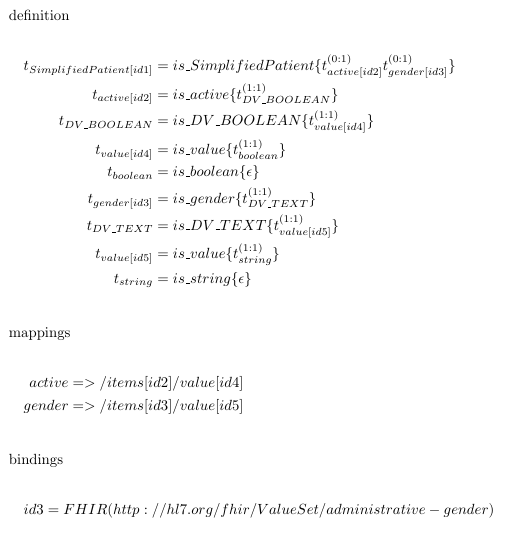
\includegraphics[scale=0.5]{./images/substitution}
  \caption{Esquema openEHR del recurso SimplifiedPatient}
  \label{fig:substitution}
\end{figure}
